% SQL2Mongo: Compiler Design Laboratory Project Report
% Build: xelatex SQL2Mongo_Project_Report.tex  (run twice so the contents page updates)
\documentclass[12pt,a4paper]{report}

\usepackage{fontspec}
\setmainfont{Times New Roman}
\setmonofont{Consolas}[Scale=0.9]

\usepackage[a4paper,margin=2.54cm]{geometry}
\usepackage{setspace}
\setstretch{1.3}
\usepackage{titlesec}
\usepackage{tabularx,longtable,array}
\usepackage{enumitem}
\usepackage{caption}
\usepackage{float}
\usepackage{needspace}
\usepackage{fancyvrb}
\usepackage{listings}
\usepackage{tikz}
\usetikzlibrary{positioning,arrows.meta,calc}
\usepackage{xurl}
\usepackage[hidelinks]{hyperref}
\urlstyle{same}

% Headings
\titleformat{\chapter}[hang]{\normalfont\Large\bfseries}{\chaptertitlename\ \thechapter:}{0.4em}{}
\titlespacing*{\chapter}{0pt}{0pt}{18pt}
\titleformat{\section}{\normalfont\large\bfseries}{\thesection}{0.6em}{}
\titlespacing*{\section}{0pt}{14pt}{6pt}

\pagestyle{plain}
\setlist{itemsep=2pt, topsep=4pt}
\captionsetup{labelfont=bf, skip=6pt}
\renewcommand{\arraystretch}{1.3}
\newcolumntype{L}{>{\raggedright\arraybackslash}X}
\newcolumntype{P}[1]{>{\raggedright\arraybackslash}p{#1}}
\setlength{\emergencystretch}{3em}

% Inline code (allows line breaks after underscores)
\newcommand{\codeus}{\textunderscore\allowbreak}
\DeclareRobustCommand{\code}[1]{\texttt{\let\_\codeus #1}}

% Code and program output
\lstset{basicstyle=\ttfamily\small\setstretch{1.0}, frame=single, framesep=4pt,
  xleftmargin=3pt, xrightmargin=3pt, columns=fullflexible, keepspaces=true,
  breaklines=true, showstringspaces=false, aboveskip=8pt, belowskip=8pt}
\fvset{fontsize=\small, baselinestretch=1, frame=single, framesep=4pt, xleftmargin=3pt, xrightmargin=3pt}

\begin{document}

% ---------------------------------------------------------------------
% Title page
% ---------------------------------------------------------------------
\begin{titlepage}
\centering
\setstretch{1.2}
\vspace*{1cm}
{\large COMPILER DESIGN LABORATORY (BCSE307P)\par}
\vspace{0.2cm}
{\large Fall Semester 2026--27\par}
\vspace{3.5cm}
{\LARGE\bfseries SQL2Mongo\par}
\vspace{0.4cm}
{\Large\bfseries A SQL-to-MongoDB Query Compiler and Execution Engine\par}
\vspace{1.5cm}
{\Large Project Report\par}
\vspace{3.5cm}
{\large Submitted by\par}
\vspace{0.5cm}
{\large
\begin{tabular}{rl}
Name: & Alan James \\
Register Number: & 24BCT0181 \\
\end{tabular}\par}
\vfill
{\large October 2026\par}
\end{titlepage}

% ---------------------------------------------------------------------
% Abstract and contents
% ---------------------------------------------------------------------
\pagenumbering{roman}
\chapter*{Abstract}
\addcontentsline{toc}{chapter}{Abstract}

Most developers learn SQL before they ever work with MongoDB, and moving to MongoDB means relearning how to write the same queries in a very different language. SQL2Mongo addresses this. It is a source-to-source compiler, written in C99, that translates SQL \code{SELECT} queries into MongoDB aggregation pipelines and runs them on an in-memory document store.

The compiler implements seven phases: lexical analysis, recursive-descent parsing with parse-tree and AST output, symbol-table-driven semantic analysis, intermediate code in three-address code, quadruple and triple form, an optimization pass, MongoDB Query Language (MQL) code generation, and execution.

The supported language covers projections, \code{WHERE} filters with \code{AND}, \code{OR} and parentheses, six comparison operators, \code{ORDER BY} and \code{LIMIT}. Each phase can be shown on its own through a command-line flag, so every intermediate form is visible during a demonstration.

The compiler is 2,370 lines of C in ten modules and uses only the C standard library. Of 19 test queries covering valid, boundary and erroneous input, 17 behave exactly as expected; the remaining 2 expose limitations in the generated target code, which are documented along with their fixes.

\tableofcontents

\cleardoublepage
\pagenumbering{arabic}

% =====================================================================
\chapter{Introduction}
% =====================================================================
SQL2Mongo lets someone who already knows SQL write a query in SQL and get the equivalent MongoDB query. It does this by applying the full compiler pipeline to the two languages, with SQL as the source and the MongoDB Query Language (MQL) as the target.

\section{Background}
Relational databases are queried with SQL, a declarative language with a fixed keyword grammar. Document databases such as MongoDB store JSON-like documents and are queried with MQL, where a query is itself a JSON structure. MongoDB's aggregation framework expresses a query as a pipeline of stages such as \code{\$match}, \code{\$sort}, \code{\$limit} and \code{\$project} \cite{mongo-pipeline}.

Both languages describe the same operations, but with different syntax and structure, so moving a query from one to the other is a translation problem.

\section{Motivation}
Most students and developers learn SQL first. It is what database courses teach, and it is the language people reach for when they think about querying data. Many of them later work on projects that use MongoDB, and they then have to learn a second, very different way of writing the same queries.

I faced this myself during my internship, where the project used MongoDB. I already knew how to write the queries I needed in SQL, but I had to work out how to express each one in MongoDB: which operator replaces \code{>=}, how \code{AND} and \code{OR} turn into nested \code{\$and} and \code{\$or} arrays, and in what order the pipeline stages must go. A small mistake in this translation does not raise an error. The query simply returns the wrong documents, or none at all.

This project grew out of that experience. Translating one query language into another is exactly what a compiler does, so I built one that takes the SQL a developer already knows and produces the equivalent MongoDB query. Because every phase prints its output, the tool also shows how each part of the SQL query maps to MongoDB, which helps someone who is learning MongoDB as well as someone who only needs the translated query.

\section{Problem Area}
The project sits in source-to-source compilation (transpilation) and database query processing. It combines classic front-end phases (scanning, parsing, semantic checks) with query-processing ideas (relational operators, query plans, predicate pushdown).

% =====================================================================
\chapter{Problem Statement}
% =====================================================================
A developer who knows SQL but has to work with MongoDB must translate every query by hand. The problem this project solves is: given a SQL \code{SELECT} query over a known schema, produce an equivalent and valid MongoDB aggregation pipeline, or report exactly where and why the query is invalid.

Hand translation from SQL to MQL has three recurring failure points:
\begin{itemize}
  \item \textbf{Operator mapping.} Each SQL comparison has a different MQL spelling (\code{>=} to \code{\$gte}, \code{!=} and \code{<>} to \code{\$ne}), and equality is written without an operator.
  \item \textbf{Logical structure.} Operator precedence must be preserved: \code{a AND b OR c} means \code{(a AND b) OR c}, which becomes an \code{\$or} array containing an \code{\$and} array.
  \item \textbf{Schema errors found late.} A misspelled field or a string compared with a number is not rejected by MongoDB. The query simply returns no documents, so the mistake goes unnoticed.
\end{itemize}
The translator must therefore check queries before generating code, and its diagnostics must point to the line and column of the fault.

\section{Requirements}
\begin{table}[H]
\centering
\begin{tabularx}{\linewidth}{|P{2.6cm}|L|}
\hline
\textbf{Type} & \textbf{Requirement} \\ \hline
Input & A SQL query, either as a \code{.sql} file path or as an inline string on the command line. \\ \hline
Output & Token table, parse tree, AST, symbol table, TAC, quadruples, triples, optimization report, MQL pipeline and query results, each selectable by a flag. \\ \hline
Functional & Reject lexical, syntax and semantic errors with a message giving the line, column and expected construct. \\ \hline
Functional & Return exit code 0 on success, 1 on a lexical or syntax error and 2 on a semantic error, so tests can be automated. \\ \hline
System & Any machine with a C99 compiler; no database server or third-party library is needed. \\ \hline
\end{tabularx}
\caption{System requirements}
\end{table}

% =====================================================================
\chapter{Objectives}
% =====================================================================
\begin{enumerate}
  \item Build a lexical analyser that recognises 11 SQL keywords, identifiers, integer, float and string literals, 7 comparison lexemes and 5 delimiters, skips comments, and tracks line and column.
  \item Build a recursive-descent parser for the query grammar that prints a concrete parse tree and builds an abstract syntax tree (AST).
  \item Build a symbol table of collections and typed fields, and use it to check collection existence, field existence and type compatibility.
  \item Generate intermediate code as three-address code, quadruples and triples.
  \item Apply query optimizations: predicate pushdown and projection pruning.
  \item Generate target MQL as a \code{db.<collection>.\allowbreak aggregate([...])} pipeline.
  \item Execute the compiled query on an in-memory document store to show the translation gives the right results.
  \item Validate the system with valid, invalid, boundary and complex test queries.
\end{enumerate}

\section{Scope}
\textbf{In scope:} single-collection \code{SELECT} queries with a column list or \code{*}; \code{WHERE} with \code{=}, \code{!=}, \code{<>}, \code{>}, \code{>=}, \code{<}, \code{<=}, \code{AND}, \code{OR} and parentheses; \code{ORDER BY} on one field, \code{ASC} or \code{DESC}; \code{LIMIT}; case-insensitive keywords.

\textbf{Out of scope:} \code{JOIN}, \code{GROUP BY} and aggregate functions, subqueries, \code{IN}, \code{LIKE} and \code{BETWEEN}, and data-changing statements (\code{INSERT}, \code{UPDATE}, \code{DELETE}). \code{NOT} is recognised by the lexer as a reserved word but is not yet part of the grammar.

% =====================================================================
\chapter{Literature Survey}
% =====================================================================
SQL-to-MQL translators already exist, but they hide their internals behind a product or a third-party parser. SQL2Mongo builds every phase by hand so each one can be shown and explained.

\section{Existing Approaches}
\begin{table}[H]
\centering\small
\begin{tabularx}{\linewidth}{|P{3.4cm}|L|L|}
\hline
\textbf{Approach} & \textbf{How it works} & \textbf{Difference from SQL2Mongo} \\ \hline
MongoDB SQL to Aggregation Mapping Chart \cite{mongo-chart} & Official reference table that maps SQL clauses to pipeline stages. & A manual guide; it performs no translation or checking. \\ \hline
mongotranslate, MongoDB BI Connector \cite{mongotranslate} & Command-line tool that shows how a SQL query is expressed as an aggregation pipeline, using a schema (DRDL) file. & Part of a large commercial product; its phases are not visible. \\ \hline
sql-to-mongo-db-query-converter \cite{russell} & Java library that converts SQL into MongoDB find, update, delete and aggregation queries. & Parsing is delegated to the JSqlParser library, so there is no hand-built lexer or parser. \\ \hline
SQL2Mongo (this project) & Hand-written lexer, parser, semantic analyser, IR generator, optimizer, code generator and executor in C. & Every phase prints its own output; schema errors are caught before code generation. \\ \hline
\end{tabularx}
\caption{Comparison with existing SQL-to-MongoDB translators}
\end{table}

\section{SQL-to-MQL Mapping}
The target forms follow MongoDB's own mapping chart \cite{mongo-chart}.
\begin{table}[H]
\centering\small
\begin{tabular}{|l|l|}
\hline
\textbf{SQL construct} & \textbf{MQL stage or operator} \\ \hline
\code{FROM t} & \code{db.t.aggregate([...])} \\ \hline
\code{WHERE} & \code{\$match} \\ \hline
\code{ORDER BY f ASC} / \code{DESC} & \code{\$sort: \{ f: 1 \}} / \code{\{ f: -1 \}} \\ \hline
\code{LIMIT n} & \code{\$limit: n} \\ \hline
\code{SELECT a, b} & \code{\$project: \{ \_id: 0, a: 1, b: 1 \}} \\ \hline
\code{=} & implicit equality \code{\{ f: v \}} \\ \hline
\code{!=}, \code{<>}, \code{>}, \code{>=}, \code{<}, \code{<=} & \code{\$ne}, \code{\$ne}, \code{\$gt}, \code{\$gte}, \code{\$lt}, \code{\$lte} \\ \hline
\code{AND}, \code{OR} & \code{\$and: [...]}, \code{\$or: [...]} \\ \hline
\end{tabular}
\caption{SQL constructs and their MQL equivalents}
\end{table}

\section{Compiler Concepts Studied}
\begin{itemize}
  \item \textbf{Phases of a compiler.} The project follows the analysis--synthesis model of Aho, Lam, Sethi and Ullman \cite{aho}: scanning, parsing, semantic analysis, intermediate code, optimization and code generation.
  \item \textbf{Recursive-descent parsing.} One function per non-terminal; operator precedence is encoded by grammar layering (\code{OR} below \code{AND} below comparisons).
  \item \textbf{Symbol tables and type checking.} The schema catalog acts as a symbol table holding each field's name and type.
  \item \textbf{Intermediate representations.} Three-address code, quadruples and triples, with relational-algebra operators \cite{codd} (scan, filter, sort, limit, project) as the instruction set.
  \item \textbf{Query optimization.} Filtering early (predicate pushdown) is a standard relational technique \cite{selinger}. MongoDB's pipeline optimization guide \cite{mongo-opt} also moves \code{\$match} ahead of \code{\$sort} and keeps \code{\$project} last.
\end{itemize}

\section{Technology Selection}
C was chosen from the course's recommended languages because it forces every data structure to be explicit \cite{kr}. The lexer and parser are written by hand rather than with Flex and Bison, so the scanning and parsing algorithms are visible in the source. Development used GCC (MinGW 6.3.0), Visual Studio Code, Git for version history and a PowerShell script for automated tests.

% =====================================================================
\chapter{System Design}
% =====================================================================
SQL2Mongo is a single-pass pipeline of seven phases. The parser builds one AST, and every later phase reads it.

\section{Architecture}
\begin{figure}[H]
\centering
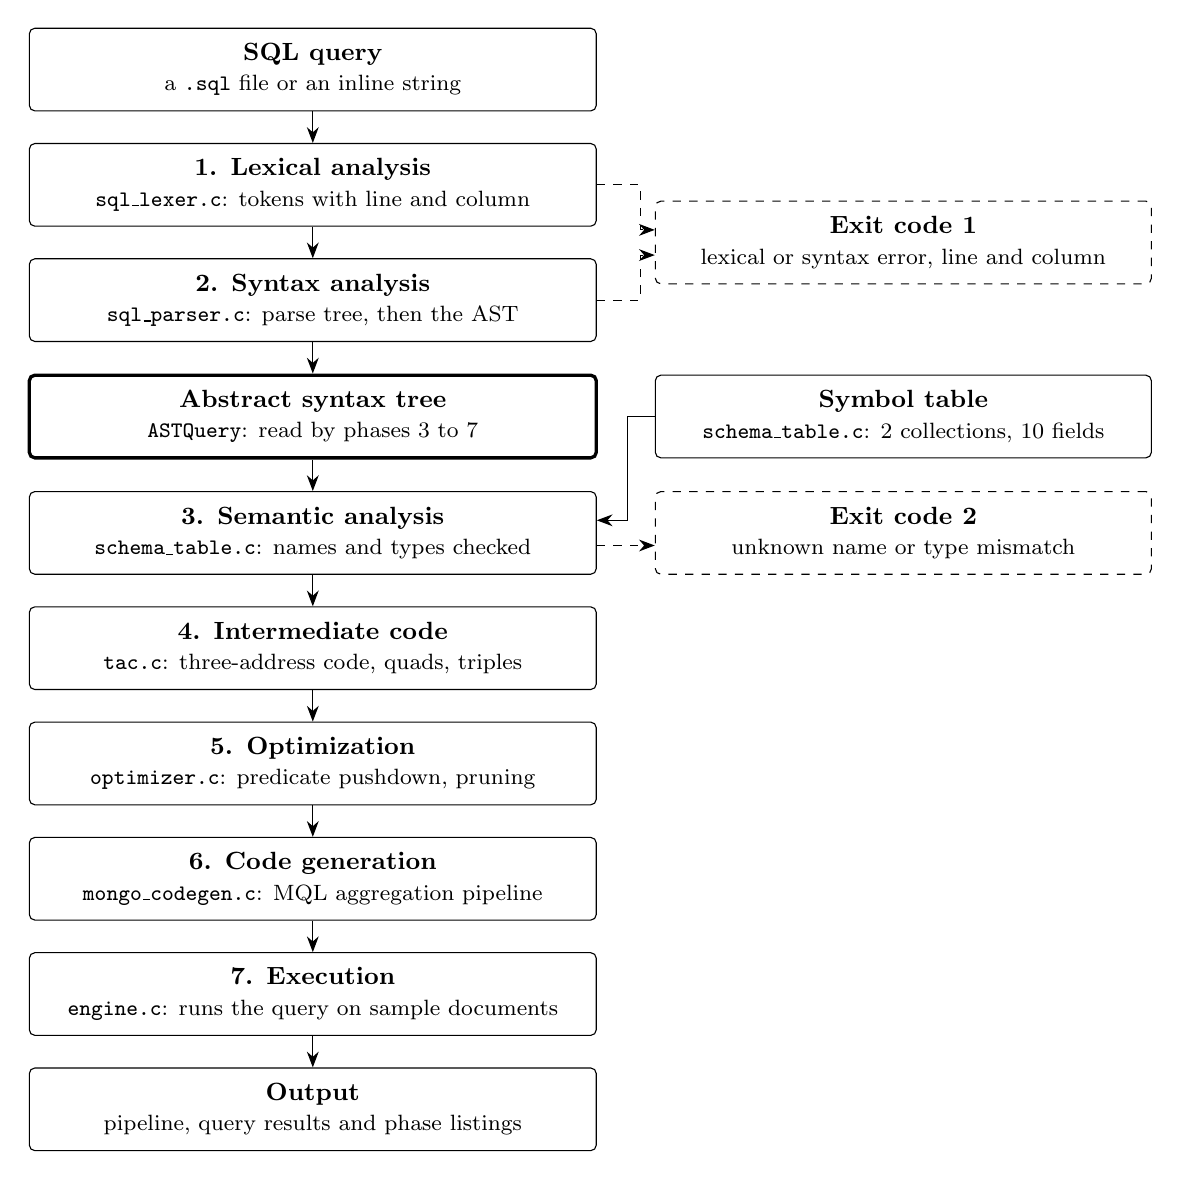
\begin{tikzpicture}[
  node distance=4mm,
  phase/.style={draw, rounded corners=2pt, minimum width=7.2cm, minimum height=1.05cm, align=center, inner sep=3pt},
  astn/.style={phase, line width=1.2pt},
  side/.style={phase, minimum width=6.3cm},
  errn/.style={side, dashed},
  flow/.style={-{Stealth[length=2mm]}},
  errflow/.style={-{Stealth[length=2mm]}, dashed},
]
\newcommand{\nm}[1]{{\small\bfseries #1}}
\newcommand{\bd}[1]{{\footnotesize #1}}
\node[phase] (in) {\nm{SQL query}\\[-1pt]\bd{a \code{.sql} file or an inline string}};
\node[phase, below=of in] (lex) {\nm{1. Lexical analysis}\\[-1pt]\bd{\code{sql\_lexer.c}: tokens with line and column}};
\node[phase, below=of lex] (par) {\nm{2. Syntax analysis}\\[-1pt]\bd{\code{sql\_parser.c}: parse tree, then the AST}};
\node[astn, below=of par] (ast) {\nm{Abstract syntax tree}\\[-1pt]\bd{\code{ASTQuery}: read by phases 3 to 7}};
\node[phase, below=of ast] (sem) {\nm{3. Semantic analysis}\\[-1pt]\bd{\code{schema\_table.c}: names and types checked}};
\node[phase, below=of sem] (ir) {\nm{4. Intermediate code}\\[-1pt]\bd{\code{tac.c}: three-address code, quads, triples}};
\node[phase, below=of ir] (opt) {\nm{5. Optimization}\\[-1pt]\bd{\code{optimizer.c}: predicate pushdown, pruning}};
\node[phase, below=of opt] (cg) {\nm{6. Code generation}\\[-1pt]\bd{\code{mongo\_codegen.c}: MQL aggregation pipeline}};
\node[phase, below=of cg] (exe) {\nm{7. Execution}\\[-1pt]\bd{\code{engine.c}: runs the query on sample documents}};
\node[phase, below=of exe] (out) {\nm{Output}\\[-1pt]\bd{pipeline, query results and phase listings}};
\node[errn] (e1) at ($(lex)!0.5!(par) + (7.5cm,0)$) {\nm{Exit code 1}\\[-1pt]\bd{lexical or syntax error, line and column}};
\node[side] (sym) at ($(ast) + (7.5cm,0)$) {\nm{Symbol table}\\[-1pt]\bd{\code{schema\_table.c}: 2 collections, 10 fields}};
\node[errn] (e2) at ($(sem) + (7.5cm,0)$) {\nm{Exit code 2}\\[-1pt]\bd{unknown name or type mismatch}};
\foreach \a/\b in {in/lex, lex/par, par/ast, ast/sem, sem/ir, ir/opt, opt/cg, cg/exe, exe/out}
  \draw[flow] (\a) -- (\b);
\draw[errflow] (lex.east) -- ++(0.55,0) |- ([yshift=1.6mm]e1.west);
\draw[errflow] (par.east) -- ++(0.55,0) |- ([yshift=-1.6mm]e1.west);
\draw[flow] (sym.west) -- ++(-0.35,0) |- ([yshift=1.6mm]sem.east);
\draw[errflow] ([yshift=-1.6mm]sem.east) -- ([yshift=-1.6mm]e2.west);
\end{tikzpicture}
\caption{Architecture of SQL2Mongo (dashed lines show error exits)}
\label{fig:arch}
\end{figure}

The phases run in the order set by \code{main.c}. The symbol table feeds only semantic analysis. Lexical and syntax errors exit with code 1 and semantic errors with code 2, so later phases never see an invalid query.

\section{Module Description}
The ten modules form three groups, coordinated by \code{main.c}:
\begin{itemize}
  \item \textbf{Front end:} \code{sql\_lexer}, \code{sql\_parser} and \code{sql\_ast} turn text into a checked syntax tree.
  \item \textbf{Middle:} \code{schema\_table}, \code{tac}, \code{optimizer} and \code{query\_plan} check meaning and build the intermediate forms.
  \item \textbf{Back end:} \code{mongo\_codegen} writes the MQL pipeline and \code{engine} executes the query.
\end{itemize}
Section~\ref{sec:modules} lists each module's size and main functions.

\section{Data Flow}
\begin{table}[H]
\centering\small
\begin{tabularx}{\linewidth}{|P{3.5cm}|L|L|}
\hline
\textbf{Phase} & \textbf{Reads} & \textbf{Produces} \\ \hline
1. Lexical analysis & Query text & Tokens (type, lexeme, value, line, column) \\ \hline
2. Syntax analysis & Tokens, pulled one at a time from the lexer & Parse tree listing and the AST \\ \hline
3. Semantic analysis & AST and symbol table & Pass, or a semantic error \\ \hline
4. Intermediate code & AST & Three-address code, quadruples, triples \\ \hline
5. Optimization & AST and IR & Optimization report \\ \hline
6. Code generation & AST & MQL \code{aggregate} pipeline \\ \hline
7. Execution & AST and the collection's documents & Result documents as JSON \\ \hline
\end{tabularx}
\caption{Data flow between phases}
\end{table}
The token table printed by \code{-{}-tokens} comes from a separate display pass. During parsing, the parser asks the lexer for each next token on demand.

\needspace{10\baselineskip}
\section{Workflow}
\begin{enumerate}
  \item The user runs \code{sql2mongo.exe} with a query file or an inline query, plus optional phase flags.
  \item \code{main.c} reads the input and loads the symbol table.
  \item The phases run in order. Each prints its listing when its flag, or \code{-{}-all}, is set.
  \item On the first error, the compiler prints the diagnostic and exits with code 1 or 2.
  \item Otherwise it prints the MQL pipeline and the query results, and exits with code 0.
\end{enumerate}

% =====================================================================
\chapter{Methodology}
% =====================================================================
The compiler was built as a single-pass, phase-by-phase pipeline around one shared data structure, the AST, with every phase observable on its own.

\section{Approach}
\begin{enumerate}
  \item \textbf{Specify the language first.} Tokens, keywords, operators and the grammar (Chapter~\ref{ch:concepts}) were fixed before any code was written, so the lexer and parser had an exact target.
  \item \textbf{One module per phase.} Each phase is a \code{.c}/\code{.h} pair with a small public interface, for example \code{lexer\_next\_token}, \code{parser\_parse}, \code{schema\_validate\_query} and \code{tac\_generate}.
  \item \textbf{AST as the contract between phases.} The parser produces an \code{ASTQuery}; every later phase reads it. This keeps phases independent and lets any of them be tested alone.
  \item \textbf{Fail fast with phase-specific diagnostics.} Compilation stops at the first error. The message names the phase, the line and column, and what was expected. The exit code tells the phase: 1 for lexical or syntax, 2 for semantic.
  \item \textbf{Make every phase visible.} Each phase has a print function and a command-line flag (\code{-{}-tokens}, \code{-{}-tree}, \code{-{}-ast}, \code{-{}-schema}, \code{-{}-tac}, \code{-{}-quads}, \code{-{}-triples}, \code{-{}-opt}, \code{-{}-mongo}, \code{-{}-run}), so a reviewer can inspect any intermediate form.
  \item \textbf{Verify by execution.} The execution engine evaluates the same AST against sample documents. Its results confirm that the generated pipeline means what the SQL query means.
  \item \textbf{Test with expected exit codes.} Each test query has a known correct exit code, and a PowerShell script runs them all and reports pass or fail.
\end{enumerate}

\section{Development Phases}
\begin{table}[H]
\centering\small
\begin{tabularx}{\linewidth}{|P{3.6cm}|L|L|}
\hline
\textbf{Phase} & \textbf{Focus} & \textbf{Outcome} \\ \hline
Phase 1: Problem definition and design & Topic, problem statement, language specification, architecture & Lexer and parser prototype with token table and validity check \\ \hline
Phase 2: Core implementation & Symbol table, semantic checks, AST, three-address code & Working front end and intermediate code generator \\ \hline
Phase 3: Final implementation and testing & Quadruples, triples, optimizer, MQL generator, execution engine, test suite & Complete seven-phase compiler with automated tests \\ \hline
\end{tabularx}
\caption{Development phases}
\end{table}

% =====================================================================
\chapter{Compiler Design Concepts Used}\label{ch:concepts}
% =====================================================================
SQL2Mongo uses eight core compiler concepts, one per phase. The running example in this chapter is the query below (test case 1).
\begin{lstlisting}
SELECT name, age FROM students WHERE age >= 20 ORDER BY age DESC LIMIT 3;
\end{lstlisting}

\section{Lexical Analysis}
The scanner (\code{sql\_lexer.c}) turns the character stream into tokens using maximal munch with one character of lookahead. The lookahead (\code{peek\_next}) separates \code{>} from \code{>=}, \code{<} from \code{<=} and \code{<>}, and \code{-} from a \code{-{}-} comment. Each token records its type, lexeme, numeric value, line and column.

\begin{table}[H]
\centering\small
\begin{tabularx}{\linewidth}{|P{3.2cm}|L|P{4.4cm}|}
\hline
\textbf{Token class} & \textbf{Pattern or lexemes} & \textbf{Token type} \\ \hline
Keywords (11, case-insensitive) & \code{SELECT FROM WHERE ORDER BY ASC DESC LIMIT AND OR NOT} & \code{TOK\_SELECT} \ldots\ \code{TOK\_NOT} \\ \hline
Identifier & \code{[A-Za-z\_][A-Za-z0-9\_]*}, not a keyword & \code{TOK\_IDENT} \\ \hline
Number literal & \code{[0-9]+(\textbackslash.[0-9]*)?} & \code{TOK\_NUMBER} \\ \hline
String literal & \code{'\ldots'} or \code{"\ldots"}, with \code{\textbackslash} escapes & \code{TOK\_STRING} \\ \hline
Comparison operator & \code{= \ != \ <> \ > \ >= \ < \ <=} & \code{TOK\_EQ}, \code{TOK\_NEQ}, \code{TOK\_GT}, \code{TOK\_GTE}, \code{TOK\_LT}, \code{TOK\_LTE} \\ \hline
Delimiter & \code{, \ ; \ * \ ( \ )} & \code{TOK\_COMMA} \ldots\ \code{TOK\_RPAREN} \\ \hline
Comment (discarded) & \code{-{}- \ldots} to end of line, \code{/* \ldots\ */} & none \\ \hline
\end{tabularx}
\caption{Token classes recognised by the lexer}
\end{table}

Keywords are recognised after an identifier is scanned: the lexeme is upper-cased and compared with the keyword list (\code{check\_keyword}). Three inputs raise a lexical error: an unknown character such as \code{@}, a lone \code{!}, and an unterminated string.

\section{Syntax Analysis}
The parser (\code{sql\_parser.c}) is a hand-written recursive-descent (LL(1)) parser: one function per non-terminal, deciding each step from the current token only. The grammar in EBNF is:
\begin{Verbatim}[fontsize=\footnotesize]
query         → select_clause from_clause [where_clause]
                [order_clause] [limit_clause] [";"] EOF
select_clause → "SELECT" ( "*" | IDENT { "," IDENT } )
from_clause   → "FROM" IDENT
where_clause  → "WHERE" or_expr
or_expr       → and_expr { "OR" and_expr }
and_expr      → primary { "AND" primary }
primary       → "(" or_expr ")" | IDENT comp_op literal
comp_op       → "=" | "!=" | "<>" | ">" | ">=" | "<" | "<="
literal       → NUMBER | STRING
order_clause  → "ORDER" "BY" IDENT [ "ASC" | "DESC" ]
limit_clause  → "LIMIT" NUMBER
\end{Verbatim}

Precedence comes from the layering: \code{primary} binds tightest, then \code{AND}, then \code{OR}. The \code{\{ \ldots\ \}} repetitions are written as \code{while} loops that fold operands to the left, so \code{a AND b AND c} becomes \code{(a AND b) AND c}. With the \code{-{}-tree} flag the parser prints the concrete parse tree:
\begin{Verbatim}
<Query>
 ├── <SelectClause>
 │    ├── Terminal: 'SELECT'
 │    └── <ProjectionList>
 │         ├── <Identifier: "name">
 │         ├── Terminal: ','
 │         └── <Identifier: "age">
 ├── <FromClause>
 │    ├── Terminal: 'FROM'
 │    └── <CollectionIdentifier: "students">
 ├── <WhereClause>
 │    ├── Terminal: 'WHERE'
 │    └── <ConditionExpression>
 │         └── <ComparisonExpr>
 │             ├── <FieldIdentifier: "age">
 │             ├── <ComparisonOp: ">=">
 │             └── <IntegerLiteral: 20>
 ├── <OrderByClause>
 │    ├── Terminal: 'ORDER'
 │    ├── Terminal: 'BY'
 │    ├── <FieldIdentifier: "age">
 │    └── Terminal: 'DESC'
 ├── <LimitClause>
 │    ├── Terminal: 'LIMIT'
 │    └── <IntegerLiteral: 3>
 └── Terminal: ';'
\end{Verbatim}

On a syntax error the parser records the first error only and reports the expected construct, for example:
\begin{Verbatim}[fontsize=\footnotesize]
Syntax error at [Line 4, Col 1]: Expected collection/table name identifier,
but found 'WHERE' (KEYWORD(WHERE))
\end{Verbatim}

\section{Abstract Syntax Tree}
The AST (\code{sql\_ast.h}) drops punctuation and keeps meaning. The root \code{ASTQuery} holds the collection name, the projection list (or a wildcard flag), an optional \code{WHERE} tree, and the \code{ORDER BY} and \code{LIMIT} settings. The \code{WHERE} tree is built from \code{ASTFilter} nodes of two kinds:
\begin{itemize}
  \item \textbf{Binary node:} a field, a comparison operator and a typed literal (\code{INT}, \code{FLOAT} or \code{STRING}).
  \item \textbf{Logical node:} \code{AND} or \code{OR} with left and right children.
\end{itemize}
Filter nodes are allocated on the heap and freed recursively by \code{ast\_free} after compilation. The \code{-{}-ast} output for the running example:
\begin{Verbatim}
SelectQueryNode
  [Projections]: name, age
  [From Collection]: students
  [Where Filter]:
    BinaryCondition: [age >= 20]
  [Order By]: age (DESCENDING)
  [Limit]: 3
\end{Verbatim}

\section{Symbol Table and Semantic Analysis}
The schema catalog (\code{schema\_table.c}) is the symbol table. Each entry is a field symbol scoped to its collection, with a data type and storage width. It holds 2 collections and 10 symbols.
\begin{table}[H]
\centering\small
\begin{tabular}{|l|l|l|l|}
\hline
\textbf{Collection} & \textbf{Field} & \textbf{Type} & \textbf{Width} \\ \hline
students & name, city, status & STRING & 64 B \\ \hline
students & age & INT & 4 B \\ \hline
students & gpa & FLOAT & 8 B \\ \hline
employees & name, department, role & STRING & 64 B \\ \hline
employees & experience & INT & 4 B \\ \hline
employees & salary & FLOAT & 8 B \\ \hline
\end{tabular}
\caption{Symbol table (schema catalog)}
\end{table}

Lookups are case-insensitive. The semantic analyser walks the AST and applies four checks in order, stopping at the first failure:
\begin{enumerate}
  \item The collection in \code{FROM} exists.
  \item Every column in \code{SELECT} exists in that collection.
  \item Every field in \code{WHERE} exists, and its type matches the literal: numeric fields take number literals, string fields take string literals.
  \item The \code{ORDER BY} field exists.
\end{enumerate}
For example, \code{WHERE age = 'twenty'} fails with \code{Semantic Type Error: Cannot compare numeric field 'age' with string literal 'twenty'}.

\section{Intermediate Code Generation}
The IR generator (\code{tac.c}) produces three-address code, then derives quadruples and triples from it. It works in two steps:
\begin{enumerate}
  \item \textbf{Condition code.} A post-order walk of the \code{WHERE} tree gives each comparison a new temporary, then combines child temporaries at each \code{AND} or \code{OR} node.
  \item \textbf{Operator chain.} Relational operators are chained in a fixed order, \code{SCAN} $\rightarrow$ \code{FILTER} $\rightarrow$ \code{SORT} $\rightarrow$ \code{LIMIT} $\rightarrow$ \code{PROJECT}, each consuming the previous temporary. Absent clauses are skipped.
\end{enumerate}
For test case 2 (\code{SELECT name, department, salary FROM employees WHERE salary >= 70000 AND department = 'Engineering' ORDER BY salary DESC}) the output is:
\begin{Verbatim}
(1)  t1 = SCAN(employees)
(2)  t2 = salary >= 70000
(3)  t3 = department == 'Engineering'
(4)  t4 = t2 AND t3
(5)  t5 = FILTER(t1, t4)
(6)  t6 = SORT(t5, salary (DESC))
(7)  t7 = PROJECT(t6, [name,department,salary])
\end{Verbatim}
Quadruples store the result temporary explicitly. Triples drop it, and later instructions refer to an earlier result by its index, such as \code{(4)}.
\begin{table}[H]
\centering\footnotesize
\setlength{\tabcolsep}{4pt}
\begin{tabular}{|c|l|l|l|l|l|l|}
\hline
 & & \multicolumn{3}{c|}{\textbf{Quadruple}} & \multicolumn{2}{c|}{\textbf{Triple}} \\ \cline{3-7}
\textbf{\#} & \textbf{Op} & \textbf{Arg1} & \textbf{Arg2} & \textbf{Result} & \textbf{Arg1} & \textbf{Arg2} \\ \hline
1 & SCAN & employees & -- & t1 & employees & -- \\ \hline
2 & \code{>=} & salary & 70000 & t2 & salary & 70000 \\ \hline
3 & \code{==} & department & 'Engineering' & t3 & department & 'Engineering' \\ \hline
4 & AND & t2 & t3 & t4 & (2) & (3) \\ \hline
5 & FILTER & t1 & t4 & t5 & (1) & (4) \\ \hline
6 & SORT & t5 & salary (DESC) & t6 & (5) & salary (DESC) \\ \hline
7 & PROJECT & t6 & name,department,salary & t7 & (6) & name,department,salary \\ \hline
\end{tabular}
\caption{Quadruples and triples for test case 2}
\end{table}

\section{Code Optimization}
The optimizer (\code{optimizer.c}) runs after IR generation and reports which optimizations apply to the query. Two are built into the shape of the IR and of the generated pipeline:
\begin{itemize}
  \item \textbf{Predicate pushdown.} \code{FILTER} always comes straight after \code{SCAN}, so \code{\$match} is always the first pipeline stage. Documents are discarded before the $O(N \log N)$ sort instead of after it.
  \item \textbf{Projection pruning.} A \code{\$project} stage is emitted only when named columns are requested, and it is placed last, as MongoDB's optimization guide recommends \cite{mongo-opt}. For \code{SELECT *} the stage is omitted altogether because it would keep every field.
\end{itemize}
Literal types (\code{INT}, \code{FLOAT}, \code{STRING}) are resolved and checked at compile time, so no type conversion is needed at run time. The grammar has no arithmetic expressions yet, so constant folding currently has nothing to fold.
\begin{Verbatim}[fontsize=\scriptsize]
1. [Predicate Pushdown]       : ENABLED & APPLIED (Filter executed before sort/projection)
2. [Projection Column Pruning]: APPLIED (2 attributes selected)
3. [Compile-Time Folding]     : APPLIED (Static type and literal resolution)
4. [Dead Stage Elimination]   : 0 redundant stages detected
\end{Verbatim}

\section{Target Code Generation}
The code generator (\code{mongo\_codegen.c}) walks the AST and emits a \code{db.<collection>.\allowbreak aggregate([...])} call. Stages appear in the order \code{\$match}, \code{\$sort}, \code{\$limit}, \code{\$project}, and only for clauses present in the query.

Filters are emitted recursively. A comparison becomes \code{\{ field: value \}} for equality or \code{\{ field: \{ \$op: value \} \}} otherwise. A logical node becomes \code{\{ \$and: [left, right] \}} or \code{\{ \$or: [left, right] \}}. Because the AST already encodes precedence, nested conditions come out correctly:
\begin{lstlisting}
SELECT name FROM students
WHERE (age > 19 AND gpa >= 3.5) OR status = 'Graduated'
ORDER BY gpa DESC;
\end{lstlisting}
\begin{lstlisting}
db.students.aggregate([
  { "$match": { "$or": [
      { "$and": [ { "age": { "$gt": 19 } }, { "gpa": { "$gte": 3.50 } } ] },
      { "status": "Graduated" }
  ] } },
  { "$sort": { "gpa": -1 } },
  { "$project": { "_id": 0, "name": 1 } }
]);
\end{lstlisting}

\section{Interpretation and Execution}
The execution engine (\code{engine.c}) is a tree-walking interpreter over the AST. It loads the collection's documents into memory, evaluates the \code{WHERE} tree recursively for each document, sorts the matches with \code{qsort} and a field comparator, applies the limit and prints the projected fields as JSON. The query above returns Diana Prince (GPA 3.95), Alice Walker (3.85) and Evan Wright (Graduated, 3.10), which is the correct answer for the sample data in Appendix~\ref{sec:data}.

\section{Error Detection and Recovery}
Errors are caught in the earliest phase that can see them. The compiler uses a stop-at-first-error strategy: it reports the fault with its position and halts with a phase-specific exit code.
\begin{table}[H]
\centering\footnotesize
\setlength{\tabcolsep}{4pt}
\begin{tabularx}{\linewidth}{|P{1.4cm}|P{2.1cm}|P{3.5cm}|L|c|}
\hline
\textbf{Phase} & \textbf{Error} & \textbf{Example input} & \textbf{Message} & \textbf{Exit} \\ \hline
Lexical & Unknown character & \code{WHERE age @ 20} & \code{Lexical error at [Line 1, Col 37]: Unrecognized or malformed token '@'} & 1 \\ \hline
Lexical & Unterminated string & \code{WHERE city = 'Seattle;} & \code{Lexical error at [Line 1, Col 40]: \ldots\ malformed token 'Seattle;'} & 1 \\ \hline
Syntax & Missing table name & \code{FROM WHERE age >= 20} & \code{Expected collection/table name identifier, but found 'WHERE'} & 1 \\ \hline
Syntax & Unbalanced parenthesis & \code{WHERE (age > 19;} & \code{Expected closing parenthesis ')', but found ';'} & 1 \\ \hline
Semantic & Unknown collection & \code{FROM teachers} & \code{Collection 'teachers' does not exist in schema catalog} & 2 \\ \hline
Semantic & Unknown column & \code{SELECT name, nonexistent\_column} & \code{Column 'nonexistent\_column' in SELECT clause is not defined} & 2 \\ \hline
Semantic & Type mismatch & \code{WHERE city = 25} & \code{Cannot compare string field 'city' with numeric literal} & 2 \\ \hline
\end{tabularx}
\caption{Error detection by phase}
\end{table}

% =====================================================================
\chapter{Implementation}
% =====================================================================
SQL2Mongo is 2,370 lines of C99 in ten modules, using only the C standard library. It builds with GCC under \code{-Wall -Wextra} with no warnings.

\section{Tools Used}
\begin{table}[H]
\centering\small
\begin{tabular}{|l|l|}
\hline
\textbf{Item} & \textbf{Used} \\ \hline
Language & C99 \\ \hline
Compiler & GCC 6.3.0 (MinGW) on Windows 11 \\ \hline
Libraries & C standard library only (\code{stdio}, \code{stdlib}, \code{string}, \code{ctype}, \code{stdbool}) \\ \hline
Editor & Visual Studio Code \\ \hline
Version control & Git \\ \hline
Test automation & PowerShell script \code{test\_all.ps1} \\ \hline
\end{tabular}
\caption{Implementation tools}
\end{table}

\section{Modules}\label{sec:modules}
\begin{table}[H]
\centering\footnotesize
\setlength{\tabcolsep}{4pt}
\begin{tabularx}{\linewidth}{|P{2.3cm}|r|L|P{4.6cm}|}
\hline
\textbf{Module} & \textbf{Lines} & \textbf{Responsibility} & \textbf{Key functions} \\ \hline
\code{sql\_lexer} & 372 & Scanner, token types, token table & \code{lexer\_next\_token}, \code{check\_keyword}, \code{lexer\_print\_all} \\ \hline
\code{sql\_parser} & 395 & Recursive-descent parser, parse-tree printer & \code{parser\_parse}, \code{parse\_or\_expr}, \code{parse\_and\_expr}, \code{parse\_primary\_filter} \\ \hline
\code{sql\_ast} & 223 & AST node types, constructors, printer, cleanup & \code{ast\_create\_binary\_filter}, \code{ast\_create\_logical\_filter}, \code{ast\_free} \\ \hline
\code{schema\_table} & 236 & Symbol table and semantic checks & \code{schema\_init}, \code{schema\_get\_field\_type}, \code{schema\_validate\_query} \\ \hline
\code{tac} & 257 & Three-address code, quadruples, triples & \code{tac\_generate}, \code{quads\_print}, \code{triples\_print} \\ \hline
\code{optimizer} & 59 & Optimization pass and report & \code{optimizer\_run}, \code{optimizer\_print\_report} \\ \hline
\code{query\_plan} & 129 & Relational query plan with per-operator cost estimates (not yet exposed by a command-line flag) & \code{plan\_generate}, \code{plan\_print} \\ \hline
\code{mongo\_codegen} & 137 & MQL aggregation-pipeline generator & \code{mongo\_codegen\_pipeline}, \code{emit\_filter\_json} \\ \hline
\code{engine} & 320 & In-memory document store and query interpreter & \code{engine\_execute\_query}, \code{eval\_filter}, \code{doc\_sort\_compare} \\ \hline
\code{main} & 242 & Command-line driver that runs the phases in order & \code{main}, \code{read\_entire\_file} \\ \hline
\textbf{Total} & \textbf{2,370} & & \\ \hline
\end{tabularx}
\caption{Source modules (lines counted over the \code{.c} and \code{.h} files)}
\end{table}

\section{Key Algorithms}
\begin{itemize}
  \item \textbf{Scanning:} a character-class switch with one-character lookahead and maximal munch; keywords found by upper-casing the identifier and comparing it with the keyword list. Linear in input length.
  \item \textbf{Parsing:} LL(1) recursive descent with one token of lookahead; left-associative operator chains built by loops. Linear in the number of tokens.
  \item \textbf{Semantic analysis:} recursive AST walk with linear symbol lookup in the catalog (10 symbols).
  \item \textbf{IR generation:} post-order traversal of the filter tree; a counter supplies fresh temporaries \code{t1, t2, \ldots}. Triples are derived by replacing each temporary with the index of the quadruple that produced it.
  \item \textbf{Code generation:} recursive emission of nested JSON for \code{\$and} and \code{\$or}.
  \item \textbf{Execution:} per-document recursive evaluation of the filter tree, \code{qsort} for \code{ORDER BY}, then limit and projection.
\end{itemize}

\section{Project Structure}
\begin{Verbatim}
compiler-project/
├── build.bat            one-step GCC build
├── test_all.ps1         automated test suite
├── data/                sample collections (students.json, employees.json)
├── examples/            test queries (4 valid, 2 error cases)
├── report/              this report (LaTeX source and PDF)
└── src/                 ten modules listed in Section 8.2
\end{Verbatim}

\section{User Instructions}
Build with \code{build.bat}, or directly:
\begin{lstlisting}
gcc -std=c99 -Wall -Wextra src/*.c -o sql2mongo.exe
\end{lstlisting}
Run on a query file or an inline query. With no flag, all phases run (\code{-{}-all}).
\begin{lstlisting}
sql2mongo.exe examples/query1_basic.sql --all
sql2mongo.exe "SELECT name, age FROM students WHERE age >= 20 ORDER BY age DESC LIMIT 2;" --mongo
\end{lstlisting}
\begin{table}[H]
\centering\small
\begin{tabular}{|l|l|}
\hline
\textbf{Flag} & \textbf{Shows} \\ \hline
\code{-{}-tokens} & Token table (lexical analysis) \\ \hline
\code{-{}-tree} & Concrete parse tree \\ \hline
\code{-{}-ast} & Abstract syntax tree \\ \hline
\code{-{}-schema} & Symbol table and semantic check result \\ \hline
\code{-{}-tac}, \code{-{}-quads}, \code{-{}-triples} & Three-address code, quadruples, triples \\ \hline
\code{-{}-opt} & Optimization report \\ \hline
\code{-{}-mongo} & Generated MongoDB pipeline \\ \hline
\code{-{}-run} & Query results from the execution engine \\ \hline
\code{-{}-all} & Every phase in order (default) \\ \hline
\end{tabular}
\caption{Command-line flags}
\end{table}
Run the automated test suite with:
\begin{lstlisting}
powershell -ExecutionPolicy Bypass -File .\test_all.ps1
\end{lstlisting}

% =====================================================================
\chapter{Testing and Results}
% =====================================================================
Of 19 test queries, 17 behave exactly as expected. The other 2 run correctly in the engine but produce MQL that a real MongoDB server would treat differently (Section~\ref{sec:findings}). All tests were run on 23 October 2026 with a fresh build of the current source.

\section{Test Cases}
Tests cover valid, boundary, lexical-error, syntax-error and semantic-error inputs. Cases 1--4, 11 and 15 form the automated suite in \code{test\_all.ps1}; all six return their expected exit codes.

{\footnotesize
\setlength{\tabcolsep}{3.5pt}
\begin{longtable}{|>{\raggedright\arraybackslash}p{0.45cm}|>{\raggedright\arraybackslash}p{1.75cm}|>{\raggedright\arraybackslash}p{4.9cm}|>{\raggedright\arraybackslash}p{2.4cm}|>{\raggedright\arraybackslash}p{3.2cm}|>{\raggedright\arraybackslash}p{1.1cm}|}
\caption{Test cases and results}\\
\hline
\textbf{\#} & \textbf{Category} & \textbf{Input (query or clause)} & \textbf{Expected} & \textbf{Actual} & \textbf{Status} \\ \hline
\endfirsthead
\hline
\textbf{\#} & \textbf{Category} & \textbf{Input (query or clause)} & \textbf{Expected} & \textbf{Actual} & \textbf{Status} \\ \hline
\endhead
1 & Valid & \code{SELECT name, age FROM students WHERE age >= 20 ORDER BY age DESC LIMIT 3;} & Exit 0; 3 documents, oldest first & Diana (23), Alice (22), Bob (21) & Pass \\ \hline
2 & Valid, \code{AND} & \code{SELECT name, department, salary FROM employees WHERE salary >= 70000 AND department = 'Engineering' ORDER BY salary DESC;} & Exit 0; \code{\$and} filter & Sarah Connor (95000), John Doe (72000) & Pass \\ \hline
3 & Valid, \code{*} and float & \code{SELECT * FROM students WHERE gpa >= 3.85;} & Exit 0; no \code{\$project} stage & 3 full documents; pipeline has \code{\$match} only & Pass \\ \hline
4 & Valid, \code{OR} & \code{SELECT name, city FROM students WHERE city = 'Seattle' OR city = 'Boston' ORDER BY name ASC;} & Exit 0; \code{\$or} filter, sorted by name & Alice, Bob, Charlie & Pass \\ \hline
5 & Complex & \code{WHERE (age > 19 AND gpa >= 3.5) OR status = 'Graduated' ORDER BY gpa DESC} & \code{\$and} nested inside \code{\$or} & Correct nesting; Diana, Alice, Evan & Pass \\ \hline
6 & Boundary & \code{WHERE age > 100} & Exit 0; empty result & 0 documents returned & Pass \\ \hline
7 & Boundary & \code{select NAME, Age from STUDENTS where AGE < 21 limit 1} (mixed case, no \code{;}) & Exit 0; 1 document & Charlie Brown returned; MQL keeps the user's casing & Partial \\ \hline
8 & Boundary & \code{LIMIT 0} & Rejected, or valid MQL & Accepted; emits \code{\$limit: 0} & Partial \\ \hline
9 & Lexical error & \code{WHERE age @ 20} & Exit 1 & Exit 1, unrecognised token \code{'@'} at col 37 & Pass \\ \hline
10 & Lexical error & \code{WHERE city = 'Seattle;} & Exit 1 & Exit 1, unterminated string reported & Pass \\ \hline
11 & Syntax error & \code{SELECT name, age FROM WHERE age >= 20;} & Exit 1 & Exit 1, expected table name, at line 4 & Pass \\ \hline
12 & Syntax error & \code{ORDER age} & Exit 1 & Exit 1, expected \code{BY} after \code{ORDER} & Pass \\ \hline
13 & Syntax error & \code{LIMIT 2 extra;} & Exit 1 & Exit 1, unexpected trailing tokens & Pass \\ \hline
14 & Syntax error & \code{WHERE (age > 19;} & Exit 1 & Exit 1, expected closing parenthesis & Pass \\ \hline
15 & Semantic error & \code{SELECT name, nonexistent\_column FROM students WHERE age = 'twenty';} & Exit 2 & Exit 2, unknown column reported first & Pass \\ \hline
16 & Semantic error & \code{WHERE age = 'twenty'} & Exit 2 & Exit 2, numeric field compared with string & Pass \\ \hline
17 & Semantic error & \code{WHERE city = 25} & Exit 2 & Exit 2, string field compared with number & Pass \\ \hline
18 & Semantic error & \code{FROM teachers} & Exit 2 & Exit 2, collection does not exist & Pass \\ \hline
19 & Semantic error & \code{FROM students ORDER BY salary} & Exit 2 & Exit 2, \code{ORDER BY} field does not exist & Pass \\ \hline
\end{longtable}
}

\section{Output Evidence}
Token table for test case 1 (\code{-{}-tokens}):
\begin{Verbatim}[fontsize=\footnotesize]
+----+-----------------------+---------------------+------+------+
| #  | Token Type            | Lexeme              | Line | Col  |
+----+-----------------------+---------------------+------+------+
| 1  | KEYWORD(SELECT)       | SELECT              | 2    | 1    |
| 2  | IDENTIFIER            | name                | 2    | 8    |
| 3  | COMMA(,)              | ,                   | 2    | 12   |
| 4  | IDENTIFIER            | age                 | 2    | 14   |
| 5  | KEYWORD(FROM)         | FROM                | 3    | 1    |
| 6  | IDENTIFIER            | students            | 3    | 6    |
| 7  | KEYWORD(WHERE)        | WHERE               | 4    | 1    |
| 8  | IDENTIFIER            | age                 | 4    | 7    |
| 9  | OPERATOR(>=)          | >=                  | 4    | 11   |
| 10 | NUMBER                | 20                  | 4    | 14   |
| 11 | KEYWORD(ORDER)        | ORDER               | 5    | 1    |
| 12 | KEYWORD(BY)           | BY                  | 5    | 7    |
| 13 | IDENTIFIER            | age                 | 5    | 10   |
| 14 | KEYWORD(DESC)         | DESC                | 5    | 14   |
| 15 | KEYWORD(LIMIT)        | LIMIT               | 6    | 1    |
| 16 | NUMBER                | 3                   | 6    | 7    |
| 17 | SEMICOLON(;)          | ;                   | 6    | 8    |
+----+-----------------------+---------------------+------+------+
Total Tokens Scanned: 17 | Lexical Errors: 0 | Status: PASS
\end{Verbatim}

Generated pipeline for test case 1 (\code{-{}-mongo}):
\begin{lstlisting}
db.students.aggregate([
  { "$match": { "age": { "$gte": 20 } } },
  { "$sort": { "age": -1 } },
  { "$limit": 3 },
  { "$project": { "_id": 0, "name": 1, "age": 1 } }
]);
\end{lstlisting}
Execution results for test case 1 (\code{-{}-run}):
\begin{Verbatim}[fontsize=\footnotesize]
Database: local_db | Collection: students | Evaluated: 5 | Returned: 3
{ "name": "Diana Prince", "age": 23 }
{ "name": "Alice Walker", "age": 22 }
{ "name": "Bob Smith", "age": 21 }
\end{Verbatim}

\section{Performance}
A complete seven-phase run averaged 48.8\,ms for test case 1 and 53.8\,ms for test case 2, over 100 runs each. A run that only prints the help text averaged 30.7\,ms, so process start-up dominates. The compiler phases and their console output account for about 18--23\,ms.

Memory use is fixed and small because every structure has a static size:
\begin{table}[H]
\centering\small
\begin{tabular}{|l|r|}
\hline
\textbf{Structure} & \textbf{Size} \\ \hline
Token & 152 B \\ \hline
AST root (\code{ASTQuery}) & 2,200 B, plus 232 B per filter node \\ \hline
IR program (TAC, quadruples, triples) & 14,352 B \\ \hline
One engine document & 3,336 B \\ \hline
Engine buffers (two arrays of 32 documents) & about 213 KB \\ \hline
\end{tabular}
\caption{Memory footprint of the main data structures}
\end{table}
Fixed limits: 32 projected columns, 32 IR instructions, 128-character lexemes, 32 documents per collection.

\section{Findings}\label{sec:findings}
\begin{itemize}
  \item \textbf{Case 7:} keywords and schema lookups are case-insensitive, but the generator copies identifiers as typed. MongoDB is case-sensitive, so \code{db.STUDENTS} and \code{"AGE"} would match nothing on a real server. Identifiers should be normalised to their catalog spelling.
  \item \textbf{Case 8:} MongoDB's \code{\$limit} stage takes a positive integer \cite{mongo-limit}, so \code{LIMIT 0} should be rejected during semantic analysis.
\end{itemize}

% =====================================================================
\chapter{Conclusion}
% =====================================================================
SQL2Mongo meets all eight objectives: it compiles a useful subset of SQL into valid MongoDB aggregation pipelines through seven hand-built phases, and it catches lexical, syntax and semantic errors before any code is generated.

The project started from a practical problem I ran into during my internship: knowing SQL well, but having to write MongoDB queries. SQL2Mongo removes the need to translate each query by hand. Its phase-by-phase output also shows how each SQL clause maps to its MongoDB form, so it doubles as a learning aid for anyone making the same switch.

The project shows that the classic compiler pipeline carries over directly to query translation. Lexing, recursive-descent parsing, symbol tables, three-address code and code generation each have a clear job, and the AST holds them together. The visible output of every phase made the compiler easy to debug and is the core of its demonstration.

Testing with 19 queries confirmed correct translation and execution for valid input, and precise diagnostics for invalid input. It also found two gaps in target-code fidelity, identifier casing and \code{LIMIT 0}, which are the first items in Chapter~\ref{ch:future}.

% =====================================================================
\chapter{Future Enhancements}\label{ch:future}
% =====================================================================
\begin{enumerate}
  \item \textbf{Target-code fidelity:} rewrite identifiers to their catalog spelling, and reject \code{LIMIT} values below 1.
  \item \textbf{Data-driven schema:} load collections from \code{data/*.json} and infer the symbol table from them, instead of the built-in catalog and documents.
  \item \textbf{Richer filters:} \code{NOT}, \code{IN} (\code{\$in}), \code{LIKE} (\code{\$regex}), \code{BETWEEN} (a \code{\$gte}/\code{\$lte} pair) and \code{OFFSET} (\code{\$skip}).
  \item \textbf{Aggregation and joins:} \code{GROUP BY} with \code{COUNT}, \code{SUM} and \code{AVG} (\code{\$group}), and \code{JOIN} (\code{\$lookup}).
  \item \textbf{Real IR optimizations:} flatten chains such as \code{a AND b AND c} into one \code{\$and} array, merge range conditions on the same field into one operator object, and drop redundant predicates.
  \item \textbf{Error recovery:} panic-mode recovery in the parser, so one run can report several syntax errors instead of only the first.
  \item \textbf{Query plan view:} expose the existing \code{query\_plan} module through a \code{-{}-plan} flag.
  \item \textbf{Live validation:} run generated pipelines on a MongoDB server through the official C driver and compare the results with the built-in engine.
\end{enumerate}

% =====================================================================
% References
% =====================================================================
\renewcommand{\bibname}{References}
\begin{thebibliography}{99}
\addcontentsline{toc}{chapter}{References}
\bibitem{aho} A.~V. Aho, M.~S. Lam, R. Sethi and J.~D. Ullman, \textit{Compilers: Principles, Techniques, and Tools}, 2nd ed. Boston: Pearson Addison-Wesley, 2006.
\bibitem{codd} E.~F. Codd, ``A relational model of data for large shared data banks,'' \textit{Communications of the ACM}, vol.~13, no.~6, pp.~377--387, 1970.
\bibitem{selinger} P.~G. Selinger, M.~M. Astrahan, D.~D. Chamberlin, R.~A. Lorie and T.~G. Price, ``Access path selection in a relational database management system,'' in \textit{Proc. ACM SIGMOD}, 1979, pp.~23--34.
\bibitem{kr} B.~W. Kernighan and D.~M. Ritchie, \textit{The C Programming Language}, 2nd ed. Englewood Cliffs: Prentice Hall, 1988.
\bibitem{mongo-chart} MongoDB, Inc., ``SQL to Aggregation Mapping Chart,'' MongoDB Database Manual. \url{https://www.mongodb.com/docs/manual/reference/sql-aggregation-comparison/}
\bibitem{mongo-pipeline} MongoDB, Inc., ``Aggregation Pipeline,'' MongoDB Database Manual. \url{https://www.mongodb.com/docs/manual/core/aggregation-pipeline/}
\bibitem{mongo-opt} MongoDB, Inc., ``Aggregation Pipeline Optimization,'' MongoDB Database Manual. \url{https://www.mongodb.com/docs/manual/core/aggregation-pipeline-optimization/}
\bibitem{mongo-limit} MongoDB, Inc., ``\$limit (aggregation stage),'' MongoDB Database Manual. \url{https://www.mongodb.com/docs/manual/reference/operator/aggregation/limit/}
\bibitem{mongotranslate} MongoDB, Inc., ``mongotranslate SQL Translation Tool,'' MongoDB BI Connector documentation. \url{https://www.mongodb.com/docs/bi-connector/current/reference/mongotranslate/}
\bibitem{russell} V. Russell, ``sql-to-mongo-db-query-converter,'' GitHub repository. \url{https://github.com/vincentrussell/sql-to-mongo-db-query-converter}
\bibitem{manual} \textit{Compiler Design Laboratory Project Instruction Manual}, BCSE307P, Fall Semester 2026--27.
\end{thebibliography}
\noindent Web sources accessed 23 October 2026.

% =====================================================================
% Appendix
% =====================================================================
\appendix
\chapter{Code Excerpts and Sample Data}

\section{Operator Precedence in the Parser}
From \code{sql\_parser.c}. \code{OR} calls \code{AND}, which calls \code{primary}, so \code{AND} binds tighter. Each loop folds operands to the left.
\begin{lstlisting}
static ASTFilter* parse_and_expr(Parser* p) {
    ASTFilter* left = parse_primary_filter(p);
    if (!left || p->has_error) return left;

    while (match(p, TOK_AND)) {
        ASTFilter* right = parse_primary_filter(p);
        if (!right || p->has_error) return left;
        left = ast_create_logical_filter(LOGIC_AND, left, right);
    }
    return left;
}

static ASTFilter* parse_or_expr(Parser* p) {
    ASTFilter* left = parse_and_expr(p);
    if (!left || p->has_error) return left;

    while (match(p, TOK_OR)) {
        ASTFilter* right = parse_and_expr(p);
        if (!right || p->has_error) return left;
        left = ast_create_logical_filter(LOGIC_OR, left, right);
    }
    return left;
}
\end{lstlisting}

\section{Post-order Three-Address Code for Filters}
From \code{tac.c}. Both children are translated first; their temporaries become the operands of the parent instruction.
\begin{lstlisting}
} else if (f->type == FILTER_LOGICAL) {
    char left_t[32];
    char right_t[32];
    generate_filter_tac(p, f->left, left_t, sizeof(left_t));
    generate_filter_tac(p, f->right, right_t, sizeof(right_t));

    snprintf(out_res, sz, "t%d", ++p->temp_count);

    const char* log_op = (f->logical_op == LOGIC_AND) ? "AND" : "OR";
    char tac_line[128];
    snprintf(tac_line, sizeof(tac_line), "%s = %s %s %s",
             out_res, left_t, log_op, right_t);

    add_tac_quad(p, log_op, left_t, right_t, out_res, tac_line);
}
\end{lstlisting}

\section{Sample Data}\label{sec:data}
All test results in Chapter~9 can be checked against these two collections.
\begin{table}[H]
\centering\small
\begin{tabular}{|l|r|r|l|l|}
\hline
\textbf{name} & \textbf{age} & \textbf{gpa} & \textbf{city} & \textbf{status} \\ \hline
Alice Walker & 22 & 3.85 & Seattle & Active \\ \hline
Bob Smith & 21 & 3.40 & Boston & Active \\ \hline
Charlie Brown & 19 & 3.90 & Seattle & Probation \\ \hline
Diana Prince & 23 & 3.95 & New York & Active \\ \hline
Evan Wright & 20 & 3.10 & Chicago & Graduated \\ \hline
\end{tabular}
\caption{The \code{students} collection}
\end{table}
\begin{table}[H]
\centering\small
\begin{tabular}{|l|l|r|r|l|}
\hline
\textbf{name} & \textbf{department} & \textbf{salary} & \textbf{experience} & \textbf{role} \\ \hline
Sarah Connor & Engineering & 95000 & 6 & Lead Dev \\ \hline
John Doe & Engineering & 72000 & 3 & Software Engineer \\ \hline
Jane Smith & Marketing & 65000 & 4 & Marketing Lead \\ \hline
Michael Scott & Management & 85000 & 10 & Regional Manager \\ \hline
Dwight Schrute & Sales & 58000 & 5 & Assistant Regional Manager \\ \hline
\end{tabular}
\caption{The \code{employees} collection}
\end{table}

\end{document}
